\subsection{Dueling Network Architectures for Deep Reinforcement Learning}
\label{sec:survey:DuelNet}
DQN알고리즘이 큰 성과를 이루며 deep Q learning에 대한 발전 속도는 굉장히 빨라졌는데, 해당 논문 또한 DQN 알고리즘을 기반한 새로운 네트워크 구조를 개발한 논문~\cite{DuelNet}이다. 
기존의 DQN은 특정 지점에서의 Q function을 추정(estimate)하기 위하여 모든 state와 action의 값을 모두 평가해야 한다. 
그러나 대부분의 경우에는 state의 가치가 중요하고 action으로 인한 가치의 변화가 극명한 경우는 많지 않다. 
따라서 해당 논문은 Figure~\ref{fig:dueling_network}과 같이 새로운 DQN 구조(dueling network)를 제안했다.

\begin{figure}[h]
\begin{center}
\begin{tabular}{c}
     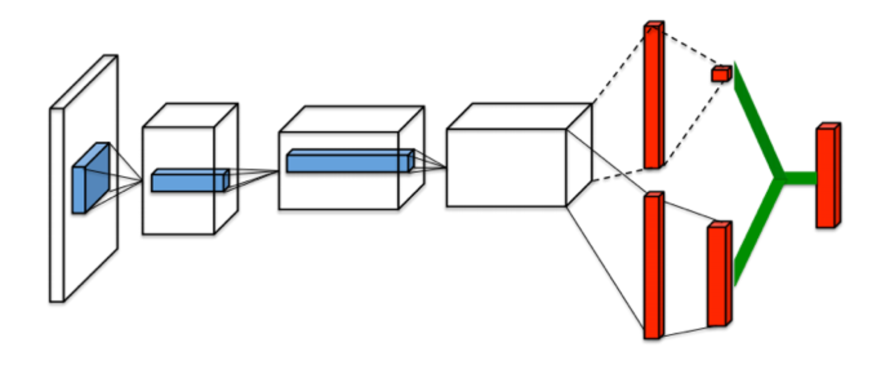
\includegraphics[width=0.45\textwidth]{FIG/DuelingNetwork.png} \\
\end{tabular}
\caption{
	Dueling Network의 구조.
}
\label{fig:dueling_network}
\end{center}
\end{figure}

앞서 말한 것처럼, 해당 논문에서의 네트워크 구조는 새로운 DQN 구조를 가지고 있는데 Q 값의 정의로부터 유도되는 한 가지 수식에서 아이디어를 얻어 탄생했다. 
해당 수식은 아래와 같다. 
\begin{align*}
	Q(s,a) = V(s) + A(s,a) \\
\end{align*}
Q 값의 의미는 현재 상태에서 행동을 취할 때 얻을 수 있는 보상의 합을 말한다. 
해당 논문에서는 이 값을 두가지로 분리하였는데 Value function(V)와 Advantage function(A)이다. 
V 값은 현재 상태에서 최선의 행동을 취했을 때 얻을 수 있는 보상의 합이고, A는 최선인 행동과 다른 행동들 사이의 보상의 차를 의미한다. 
이러한 구조를 자세히 보면 Q 값을 추론하는 것을 두 가지로 분리해서 생각한 것인데, 현재 상태가 좋은지 나쁜지를 V 값으로 추론하고 그 중에서 어떤 행동을 고를지를 A 값을 이용하여 추론한다. 
따라서 V 값은 바이어스 같은 역할을 하고 V를 중심으로 좋고 나쁨을 A 값을 이용하여 추론하게 되는 것이다. 

Dueling Network 또한 DQN과 마찬가지로 게임 이미지를 입력 값으로 받아 Q 값을 추정(estimate)한다. 
해당 논문에서 제시한 알고리즘은 Atari 게임에서 DQN을 더불어 다른 메소드보다 높은 성능을 보였다.

앞서 말한 것과 같이 우리의 프로젝트 또한 Atari 게임과 비슷한 환경을 가지고 있기 때문에 해당 알고리즘을 사용하여 성능을 높일 수 있을 거라 판단한다. 
또한 논문에서는 해당 알고리즘은 기존에 존재하는 여러 알고리즘(DQN, SARSA)에서도 사용될 수 있다고 설명한다. 
따라서 프로젝트에서 DQN으로 시도를 할 것을 염두하고 있기 때문에 DQN 혹은 DDQN을 사용할 경우 해당 알고리즘을 추가하여 손쉽게 성능을 높이기 위한 추가적인 시도를 할 것이다.
